As the number of news articles published each day grows, it becomes impossible to manually examine them all to learn about events happening in the world. The field of Event Detection arose as a subfield of Information Retrieval \citep{information-retrieval-2, information-retrieval} and Topic Detection and Tracking \citep{tdt, tdt-2} with a goal to aid the users by automatically discovering important events in document collections.

More precisely, given a stream of text documents published over a certain time period, the task is to analyze them and output a collection of events that happened in the world during the period. An event is loosely defined as \textit{something happening in a certain place at a certain time} \citep{retrospective-online-study}.

In this thesis, we chose to modify an approach introduced by \cite{event-detection}, which is a retrospective \footnote{Discussed in \autoref{sec:related-event-detection}} method relying on event representation through keywords. These keywords are semantically related words with a similar temporal characteristic. The assumption is that related words frequently co-occurring during the same time period are representative of the same events that happened at that time.

We attempt to modify this method in various ways to obtain events of higher quality. We aim for a small number of events comprised of highly relevant keywords without any underlying noise. These events should have a clear interpretation, and not be redundant of each other. To achieve this, we introduce a word embedding-based measure of word similarity, which will be discussed in \autoref{chap:related-work} and \autoref{chap:data-preprocessing} in more detail.

Once we obtain the events represented in terms of keywords, we query the document collection to also obtain the documents related to the events. We then use these documents and keywords together to generate human-readable annotations that reveal more information about the events.

The rest of the thesis is organized as follows. First, in \autoref{chap:related-work}, we discuss related work. Then, in \autoref{chap:data-preprocessing}, we describe the document collection used for evaluation and the preprocessing steps taken.

In \autoref{chap:word-analysis}, we describe the original paper's procedure used to extract temporal characteristics of the individual words. These characteristics are then examined to reveal a subset of words which may be related to certain events, as opposed to generally appearing noisy words, so called \textit{stopwords}.

Then, in \autoref{chap:event-detection}, we proceed to the event detection itself. Here, we describe the original method, its modification relying on word embedding and also propose an alternative algorithm for event detection.

Although a set of related keywords provides a concise event representation, it is not particularly readable to the user. In \autoref{chap:document-retrieval}, we follow by interpreting each keyword set as a query to the document collection. This allows us to employ Information Retrieval techniques to obtain documents relevant to each event.

Since the number of documents may be still too high, we also generate a short annotation for each event. The user can quickly skim through these annotations to get an idea what the events are about, and decide which of them are worth a closer examination. This will be addressed in \autoref{chap:event-annotation}.

Finally, we evaluate our method and compare it to the original paper in \autoref{chap:evaluation}. We then conclude the thesis in \autoref{chap:conclusion}.

\begin{figure}[H]
  \centering
  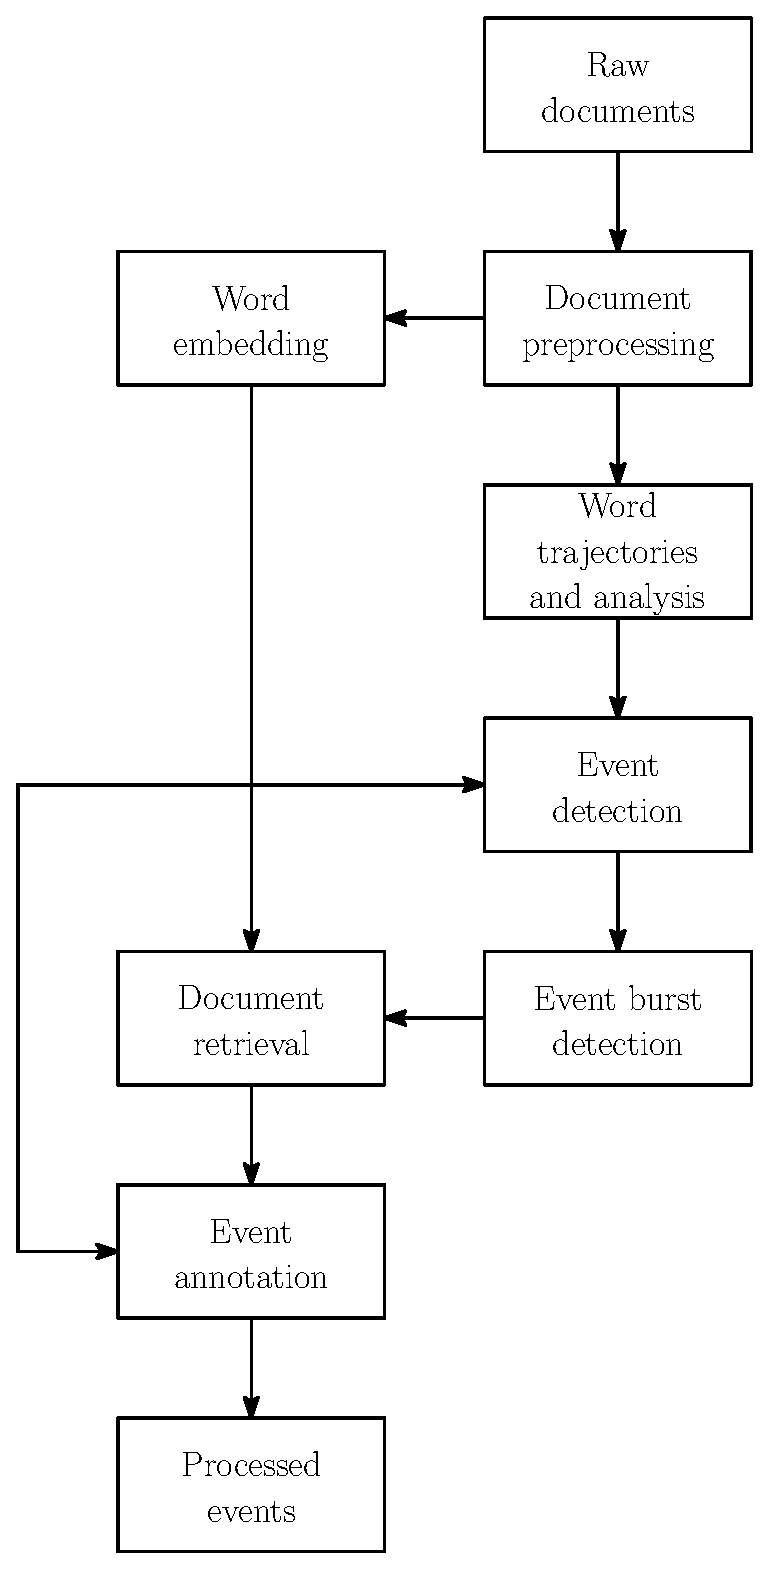
\includegraphics[height=0.5\paperheight]{diagram}
  \caption{Schematic representation of our method.}
  \label{fig:diagram}
\end{figure}